\documentclass{article}

% Language setting
% Replace `english' with e.g. `spanish' to change the document language
\usepackage[english]{babel}

% Set page size and margins
% Replace `letterpaper' with `a4paper' for UK/EU standard size
\usepackage[a4paper,top=2.5cm,bottom=2cm,left=2.5cm,right=2.5cm,marginparwidth=1.75cm]{geometry}

% Useful packages
\usepackage{amsmath}
\usepackage{graphicx}
\usepackage{subcaption} % For subfigures
\usepackage[colorlinks=true, allcolors=blue]{hyperref}
\usepackage{float}
\usepackage{titling}
\setlength{\droptitle}{-5em} 

\title{\textbf{Machine Learning: Exercise 1}}
\author{\textit{Amélie Assmayr (12007770)} \and
        \textit{Konstantinos Damanakis (12106343)} \and
        \textit{Teresa Schuch (12007762)}}
\date{}

\begin{document}
\maketitle
\vspace{-20pt}

\section{Introduction}
This report outlines the experimental design of the application of different classification algorithms across four diverse datasets. The goals is to show the trends in classifier performance, based on dataset properties like size and dimensionality, as well as the impact of preprocessing steps like scaling and different parameter settings.

The report is structured as followed: In Section 2 we introduce the chosen classifier and shortly explain their functionality. Section 3 describes the performance metrics used to evaluate each model across different configurations. Section 4 details the main characteristics of each datasets, the preprocessing steps applied and presents the evaluation results. Finally, in Section 5 discusses the main findings and insights drawn from the analysis.

\section{Classifiers}
We selected three distinct classifiers: an ensemble method (Random Forest), a margin-based method (SVM), and a distance-based method (KNN). This diverse selection will us help compare the effect of diffent classifiers better. Since we had a dataset where the target variable was non-binary we had to make sure to choose classifiers that can detect that e.g. no logistic regression.

\subsection{K-nearest-neighbors}
k-NN is a simple and intuitive classifier based on the proximity of instances. We wanted to see how it would handle the big datasets since it can be slow with large datsets. k-NN is also sensitive to the scale of the data, so it can help us identify the effect of scaling well. It works by finding the k training samples that are closest to the test sample, based on a distance metric (commonly Euclidean distance), and then making predictions based on the majority class of the neighbors.

\subsection{Random Forest}
Random Forest (RF) is a margin-based method.It works by finding a hyperplane that best separates the data points of different classes. SVM aims to maximize the margin between the closest points of each class, known as the support vectors. We chose this algorithm because particularly effective for classification tasks in high-dimensional spaces. It can also handle non-linear relationships well.  It can be computationally expensive so it is interesting to see how it will handle the big datasets. 


\subsection{Support Vector Machines}
Suport VEctor Machine (SVM) is an ensemble  method based on decision trees. It builds multiple decision trees during training and combines their prediction for more accurate and stable results. We chose this algorithm because it is good at handling both numerical and categorical data, making it a robust choice for diverse datasets. Furthermore due to its functionality Random Forests are resistant to overfitting, requires minimal preprocessing and offers offers flexibility through parameter tuning. This makes it useful also for complex and large datasets.

\section{Performance Measures}
In order to ensure that the performance of the classifiers can be meaningfully compared, the following steps were taken:
\begin{itemize}
    \item \textbf{Dataset:} The same train/test splits were used across all classifiers to ensure consistency across all experiments.
    \item \textbf{Parameter changes:} To compare how one hyperparameter affects the outcome, only a single hyperparameter was changed at a time.
    \item \textbf{Baseline comparison:} The classifiers can be compared based on their baseline performance where no hyperparameters are set.
\end{itemize}

\subsection{Training time}
\subsection{Accuracy}
$\text{Formula} = \frac{TP + TN}{TP + TN + FP + FN}$

Accuracy measures the proportion of correctly classified instances out of all instances. While it’s easy to interpret, it can be misleading, especially in imbalanced datasets, because it doesn't distinguish between false positives and false negatives.

\subsection{Precision}
$\text{Formula} = \frac{TP}{TP + FP}$

Precision measures how many of the positive predictions were actually correct and therefore measures the model’s ability to precisely identify relevant instances within the data. Either by class or averaged across all classes.

\subsection{Recall}
$\text{Formula} = \frac{TP}{TP + FN}$

Recall measures how many true positive cases the model was able to identify. Either by class or averaged
across all classes.

\subsection{F1-score}

$\text{Formula}  = 2 \times \frac{\text{Precision} \times \text{Recall}}{\text{Precision} + \text{Recall}}$

The F1-score balances precision and recall. It thereby gives accurate results even if the dataset is skewed towards certain target classes. It might however be more difficult to immediately understand the score.

\section{Datasets}
We used four datasets to evaluate different classification methods. In addition to the \textit{Congressional Voting} and \textit{Amazon Reviews} datasets, which were required, we also selected the \textit{Machine Failure} and \textit{Road Traffic Accident} datasets. We ensured that all the datasets were diverse to assess how their different properties would affect the algorithms. \newline
First, the number of dimensions varies among the datasets. The \textit{Amazon Reviews} dataset has 750 instances and 10,002 variables, making it the dataset with the highest dimensionality. The dataset with the largest number of instances is the \textit{Road Traffic Accident} dataset, containing 12,290 instances and 32 variables. The \textit{Machine Failure} dataset includes 944 instances with 10 variables, while the smallest dataset is the \textit{Congressional Voting} dataset, with 218 samples and 18 dimensions.\newline
All the datasets, except for the \textit{Road Traffic Accident} dataset, have a binary target variable. The \textit{Road Traffic Accident} dataset has a multivariate target variable. Additionally, the \textit{Road Traffic Accident} and \textit{Congressional Voting} datasets contained missing values, necessitating preprocessing. The other two datasets had no missing values.\newline
More details about the datasets and their preprocessing are provided in their respective subsections.

PLOTS: Correlation and Barplot of Target

\subsection{Congressional Voting}
This dataset contains the voting records of U.S. House of Representatives members. It has 18 columns and 218 observation, making it one of the smaller datasets used. It includes voting data on 16 key issues, where each vote is recorded as "Yes," "No," or "Unknown." The target variable indicates whether each representative is a Democrat or Republican. Additionally, there is an ID column for each representative.


\subsubsection{Preprocessing}
First, a LabelEncoder is applied to convert the categorical variables into a binary format.  For the target variable, Democrats are encoded as 0 and Republicans as 1.  n the vote columns, 'no' is encoded as 0 and 'yes' as 1. Any 'unknown' values are replaced with NaN to mark them as missing. Next, rows with more than half of their values missing are removed from the dataset. The remaining missing values are then imputed by filling them with the most frequent value in each column. Since the dataset consists only of binary data, there is no need for additional transformations like scaling or outlier handling. 

\subsubsection{Results}

\subsection{Amazon Reviews}
\subsubsection{Preprocessing}
\subsubsection{Results}

\subsection{Road Traffic Accidents}
The \textit{Road Traffic Accident} dataset contains records of road traffic accidents that occurred between 2017 and 2020 in Addis Ababa, Ethiopia. This dataset provides detailed information about the severity of accidents, the number and characteristics of the involved vehicles and individuals, the areas where the accidents occurred, and other relevant factors.
We selected this dataset because it addresses a critical public safety issue. Analyzing this data can help predict the severity of road accidents, which may, in turn, identify key causes and factors contributing to road safety. Additionally, this analysis could be valuable for stakeholders such as insurance companies and car rental services by providing insights into accident risks based on factors like the driver, vehicle type, timing, and location.
\newline
Missing data can be observed in 16 of the 32 features. Overall there are s 20.057 missing values. In the following table all attributes, their datatype(r=ratio quantity, o=ordinal, n=nominal), the number of unique elements for categorical variables and the number of missing values can be seen :
\setlength{\tabcolsep}{1pt} % Reduce padding in table cells
\begin{table}[H]
    \parbox{.5\linewidth}{
        \begin{tabular}{l@{}c@{}c@{}c}
            \textit{\textbf{Variable}} & \textbf{Type} \hspace{0.3em} & \textbf{Unique} \hspace{0.3em} & \textbf{Missing}\\\hline
            \textit{Time} & r & / & / \\
            \textit{Day of Week} & n & 7 & /\\
            \textit{Age of Driver} & o & / & /\\
            \textit{Sex of Driver} & n & 3 &/ \\
            \textit{Educational Level} & n & 7 & 741\\
            \textit{Vehicle-Driver Relation} & n & 4 & 579 \\
            \textit{Driving Experience} & o & / & 829\\
            \textit{Vehicle Type} & n & 17 & 950\\
            \textit{Vehicle Owner} & n & 4 & 482\\
            \textit{Vehicle Service Year} & r & / & 3928\\
            \textit{Defect of Vehicle} & n & 3 & 4427\\
            \textit{Accident Area} & n & 14 & 239\\
            \textit{Lanes or Medians} & n & 7 & 385\\
            \textit{Road Alignment} & n & 9 & 142\\
            \textit{Junction Type} & n & 8 & 887\\
            \textit{Road Surface Type} & n  & 4 & 172
        \end{tabular}
    }
    \hfill
    \parbox{.5\linewidth}{
        \begin{tabular}{l@{}r@{}c@{}c}
            \textit{\textbf{Variable}} & \textbf{Type} \hspace{0.3em} & \textbf{Unique} \hspace{0.3em} & \textbf{Missing}\\\hline
            \textit{Road Surface Condition} & n & 4 & 172\\
            \textit{Light Condition} & n & 4 & /\\
            \textit{Weather Condition} & n & 9 &/\\
            \textit{Collision Type} & n & 10  & 155\\
            \textit{Number of Vehicles} & r & / &/\\
            \textit{Number of Casualty} & r & / &/\\
            \textit{Vehicle Movement} & n & 13 & 308\\
            \textit{Casualty Class} & n & 4 &/ \\
            \textit{Sex of Casualty} & n & 3 & / \\
            \textit{Age of Casualty} & r & / & /\\
            \textit{Casualty Severity} & o & 4 & / \\
            \textit{Work of Casualty} & n & 7 & 3198\\
            \textit{Fitness of Casualty} & n & 5 & 2635 \\
            \textit{Pedestrian Movement} & n & 9 &/ \\
            \textit{Cause of Accident} & n & 20 & /\\
            \textit{Severity of Accident} & n & 3 & /
        \end{tabular}}
\end{table}


\subsubsection{Preprocessing}
When reading in the data, all variables were initially imported as character variables, so we first converted them to their appropriate types. All numeric variables were converted to numeric, ordinal variables were transformed into ordered factors, and the time variable was converted into a time format. Additionally, all variables containing values such as "NA," "", "NULL," "unknown," "Unknown," or "na" were treated as missing values. To simplify handling, the hour was extracted from the \textit{Time} variable, as it originally had many unique values.
We started our preprocessing by calculating the correlation of your variables.\newline
We began our preprocessing by calculating the correlation between variables. For numeric and ordered variables, we used Spearman correlation, while for other variables, we calculated Cramér's V. Due to the large number of variables, it is impractical to show a correlation plot for all of them. Instead, the correlation of the numeric and ordered variables is presented in Figure \ref{fig:cor_RTA}:
\begin{figure}[H]
\centering
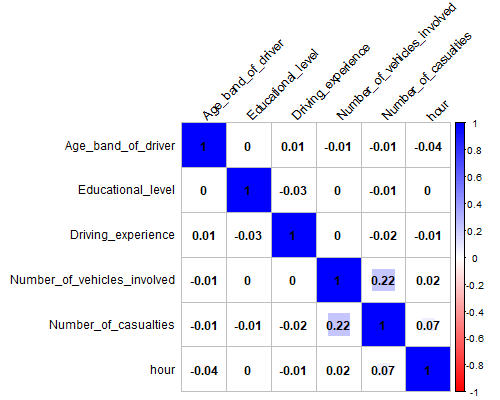
\includegraphics[width=0.8\linewidth]{plots_correlation_num_RTA.png}
\caption{\label{fig:cor_RTA} Correlation plot of some variables}
\end{figure}

As shown in Figure \ref{fig:cor_RTA}, \textit{Number of Casualties} and \textit{Number of Vehicles Involved} have a small correlation. Additionally, \textit{Area Accident Occurred} and \textit{Owner of Vehicle}, as well as \textit{Road Alignment} and \textit{Area Accident Occurred}, exhibit small correlations. Conversely, \textit{Weather Conditions} and \textit{Road Surface Conditions}, as well as \textit{Pedestrian Movement} and \textit{Casualty Class}, have high correlations.
Next, I addressed missing values. Rows with more than one-third of their values missing were removed, resulting in the deletion of 26 rows, which had no significant impact. Columns with more than half of their values missing were also removed. Furthermore, the \textit{Time} variable was excluded since it was replaced by the \textit{Hour} variable. Notably, many recorded times ended in "0" or "5" (e.g., 12:00 and 12:05) compared to times like 12:04, indicating that time values were often rounded.
Finally, I removed the following variables due to high percentages of missing values and limited relevance to the question or their lack of correlation with \textit{Accident Severity}: \textit{Age Band of Casualty}, \textit{Casualty Severity}, \textit{Work of Casualty}, and \textit{Fitness of Casualty}.
\newline
To impute the missing values, we applied different approaches based on the nature of the variables and the amount of missing data. The variables \textit{Sex of Driver}, \textit{Vehicle Driver Relation}, \textit{Owner of Vehicle}, \textit{Area Accident Occurred}, \textit{Lanes or Medians}, \textit{Road Alignment}, \textit{Road Surface Type}, \textit{Type of Collision}, \textit{Vehicle Movement}, and \textit{Cause of Accident} were imputed using their mode. This approach was chosen because these variables had relatively few missing values and no strong correlations with other variables.

For \textit{Type of Junction}, \textit{Educational Level}, and \textit{Age Band of Driver}, the missing values were imputed using proportional allocation to reflect the original distribution of the data.

For variables with higher correlations, we used imputation based on related variables. For example, \textit{Weather Conditions} was imputed based on \textit{Road Surface Conditions}. If \textit{Road Surface Conditions} was "Snow," \textit{Weather Conditions} was imputed as "Snow." If \textit{Road Surface Conditions} was "Flood over 3cm deep" or "Wet or Damp," \textit{Weather Conditions} was imputed as "Raining," and for other cases, it was imputed as "Normal." Similarly, missing values in \textit{Casualty Class} were imputed based on \textit{Pedestrian Movement}, and missing values in \textit{Educational Level} were imputed based on \textit{Vehicle Driver Relation}.

\subsubsection{Target variable}
The target variable is \textit{Severity of Accident}, which is categorized into three classes: \textit{Slight Injury}, \textit{Serious Injury}, and \textit{Fatal Injury}. While the severity could technically be considered an ordinal variable, we treated it as nominal and framed the task as a multiclass classification problem.

The following plot shows the distribution of these classes. It is evident that the classes are unevenly distributed. Most accidents fall under the \textit{Slight Injury} category, followed by \textit{Serious Injury}, while only a small number of accidents are classified as \textit{Fatal Injury}. This class imbalance is a critical consideration, and methods such as bootstrapping or oversampling could be employed to address it effectively.

\begin{figure}[H]
\centering
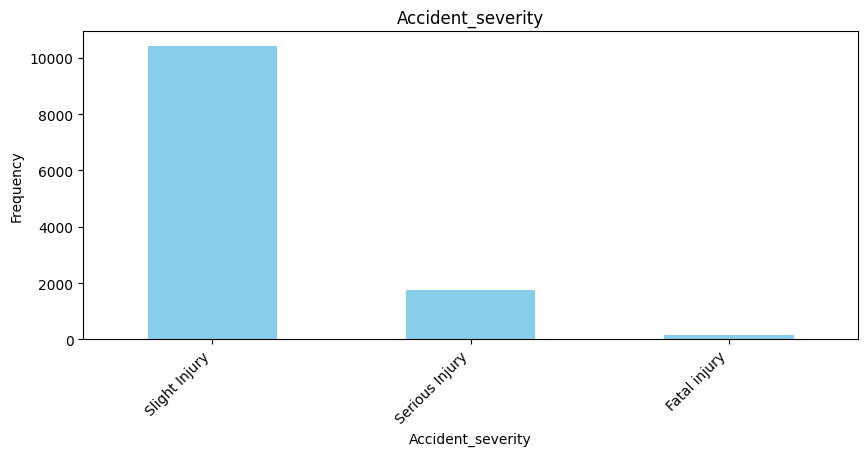
\includegraphics[width=1\linewidth]{Accident_severity.png}
\caption{\label{fig:bar:severity} Barplot of Accident Severity}
\end{figure}



\subsubsection{Results}

\subsection{Machine Failure}
The \textit{Machine Failure} dataset contains sensor data collected from various machines, including a range of sensor readings and records of machine failures. The primary goal of this dataset is to predict whether a machine will fail or not.

We selected this dataset because it addresses an important issue in industrial settings. Unexpected machine failures can result in significant financial losses for companies. Predicting potential failures in advance allows for timely maintenance and replacement, ensuring operational efficiency and reducing downtime.

\noindent There are no missing values in this dataset. The following table lists all the attributes, their data types (\textit{r} = ratio quantity, \textit{o} = ordinal, \textit{n} = nominal), and the number of unique elements:

\setlength{\tabcolsep}{1pt} % Reduce padding in table cells
    \begin{table}[H]
        \begin{tabular}{l@{}c@{}c@{}c}
                \textit{\textbf{Variable}} & \textbf{Type} \hspace{0.3em} & \textbf{Unique} \hspace{0.3em} \\\hline
                \textit{footfall } & r & 99 \\
                \textit{tempMode} & r & 8 \\
                \textit{AQ} & r & 7 \\
                \textit{USS} & r & 7 \\
                \textit{CS} & r & 7 \\
                \textit{VOC} & r & 7  \\
                \textit{RP} & r & 71 \\
                \textit{IP} & r & 7 \\
                \textit{Temperature} & r & 24 \\
                \textit{fail} & r & 2 
        \end{tabular}
    \end{table}

While the data types in the \textit{Road Traffic Accident} were divers with mainly charcter variables here we have only numeric variables. All the variables are integers.

\subsubsection{Preprocessing}
Since there were no missing values preprocessing was not really necessary, but we did look at the correlation of the variables to see if some might be redundant. We used the pearson correlation. AS we can see the dataset has some high correlations especially beween \textit{VOC} and \textit{fail} and between \textit{VOC} and \textit{AQ}.

\begin{figure}[H]
\centering
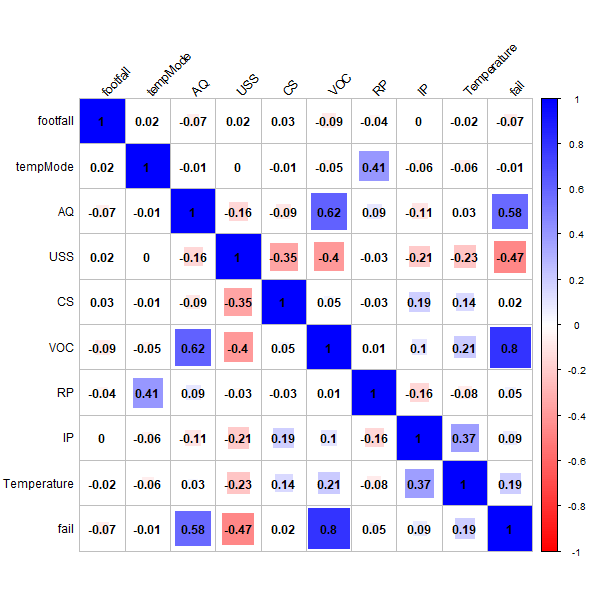
\includegraphics[width=0.8\linewidth]{plots_correlation_Machine.png}
\caption{\label{fig:cor_machine} Correlation plot}
\end{figure}


\subsubsection{Results}


\section{Discussion of Findings}



\section{Notes}

\end{document}